\section{Discussion} \label{sec:discuss}
For the simulated data, the results are generally unsurprising. 
The more a phylogeny adheres to a molecular clock, the more accurate predictions made from it will be -- the simulated data is very well informed, and the phylogeny and its clock are very well resolved by the maximum likelihood tree estimate. 
Since latency is akin to ``pausing'' the evolution of a sequence, and evolution is assumed to be clock-like when sequences are not ``paused'', it's also not surprising that the latent simulated data could also be reconstructed with low error. 

The results from the {\em plasma} data-set are also expected. 
Each patient from our plasma data-set showed evidence of a molecular clock, so the ability to reconstruct known dates came as no surprise. 
However, the reconstruction error was higher than that of the simulated data, which is expected for data that come from a biological process that is not fully understood.

Quantitatively, it's difficult to assess the accuracy of the reconstructions within the {\em mixed} data set. 
Many patients show evidence of latency in their regression plots (see the regression plot of \ref{fig:results2} D) but it's unclear what the general pattern is (if any) for the distribution of the error metrics. 
Moreover, it's not possible to know the actual error for this data set, as that would require us to know the date at which a sequence became latent. 
We also observed an interesting sigmoidal pattern in many of the patients in this case.
However, we do note that most treated patients failed the hypothesis testing, implying that samples after treatment should be ignored in any analysis with this methodology.

Typically, we also observed that the rooting method had very little effect on the errors (the supplemental material has figure \ref{fig:results} replicated for RTT rooting). 
We did, however, identify a case in which RTT rooting fails over outgroup rooting.
Figure \ref{fig:degenerate_example}, shows an example of this. 
Specifically, it's possible for the calibration dates to provide insufficient data to resolve the root of the tree. 
We theorize that this is, for patient 820, because their calibration samples are strongly localized in time, which allows too much freedom (temporally) over the possible roots of the tree. 

\begin{figure*}[!ht] \label{fig:degenerate_example}
	\centering
	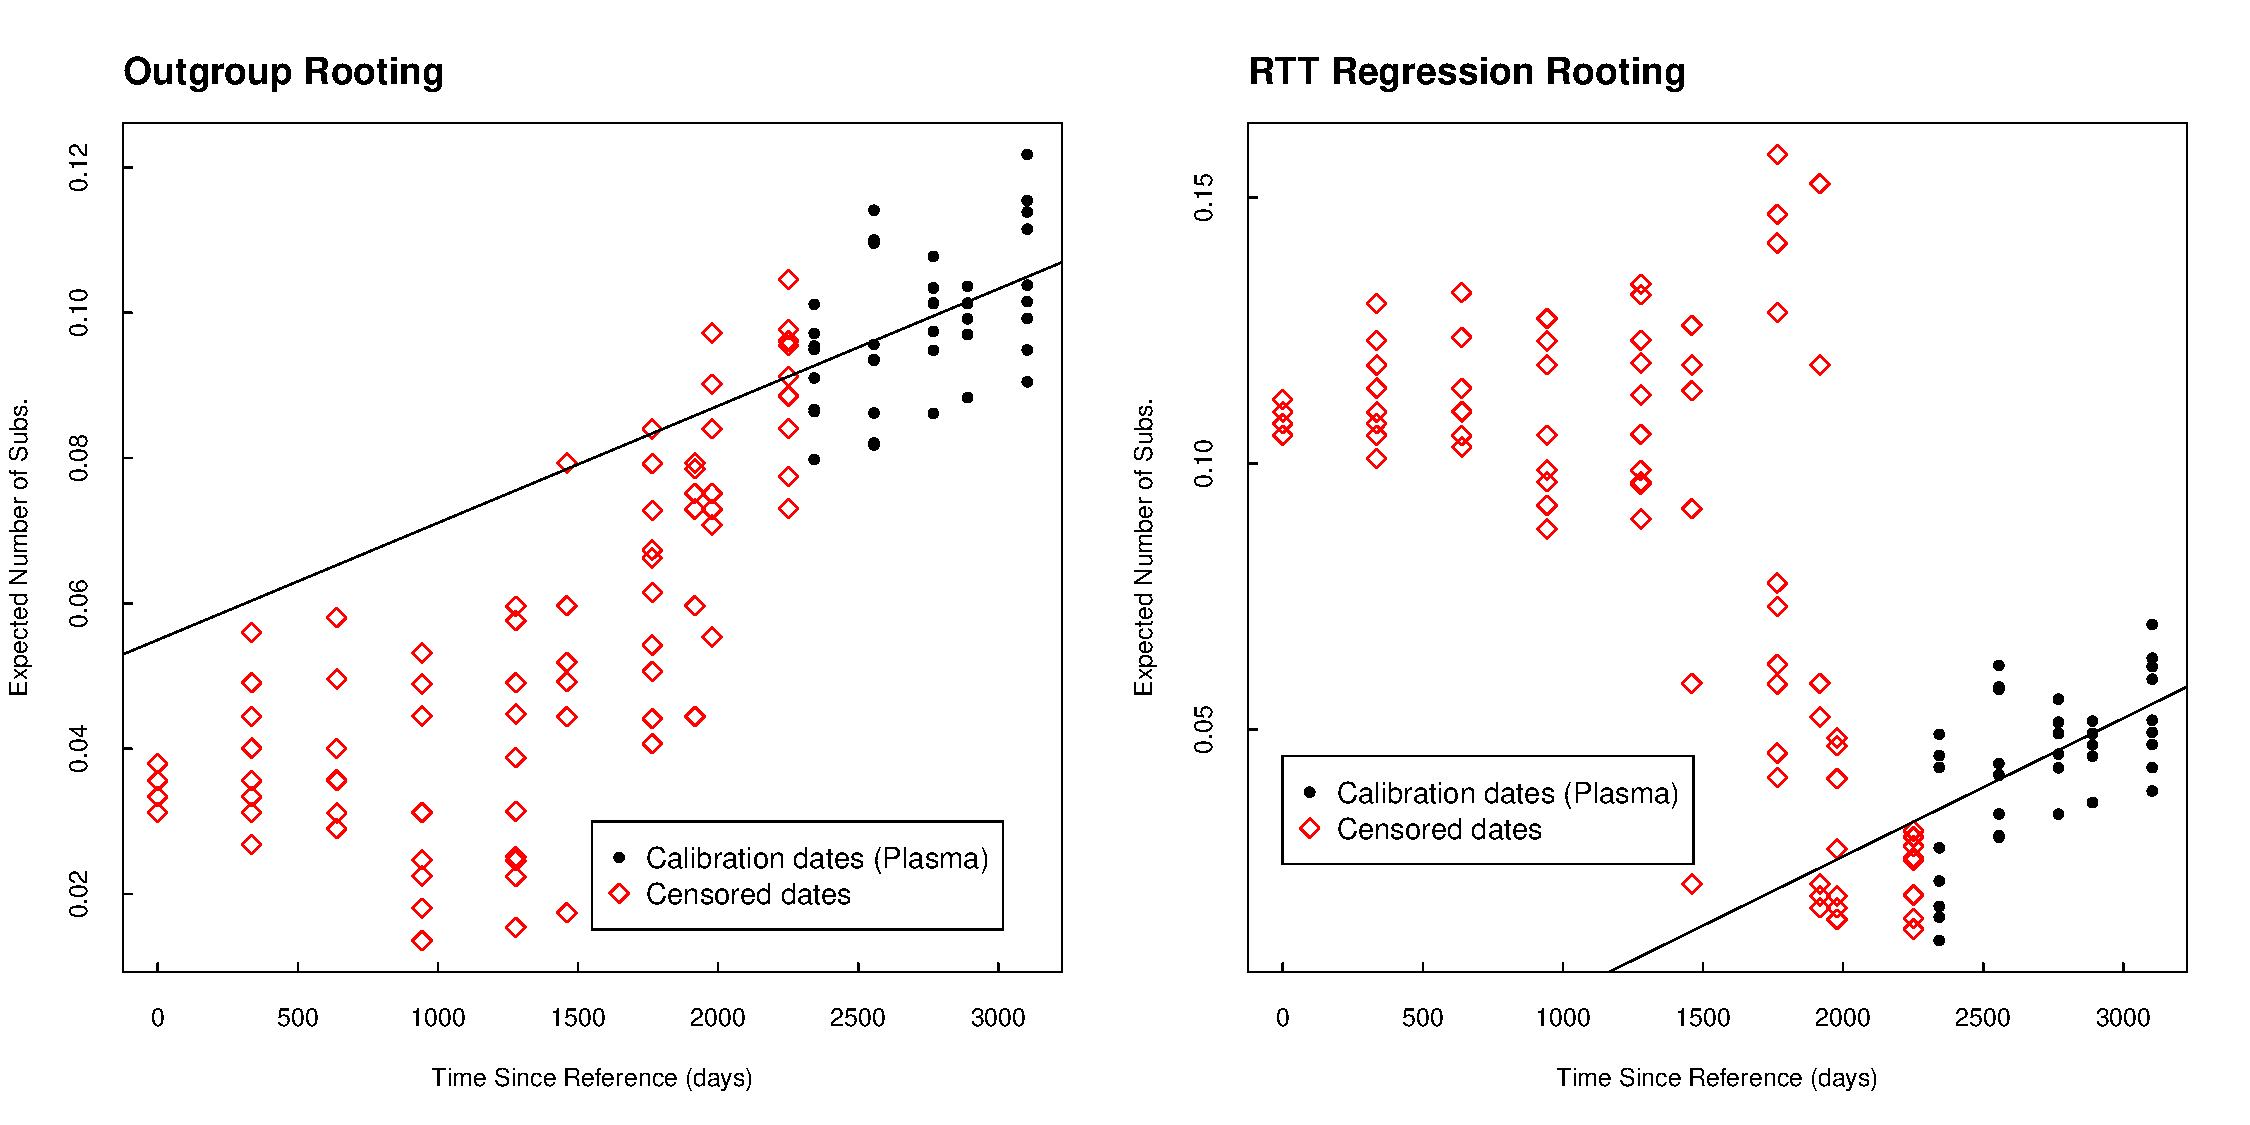
\includegraphics[scale=0.425]{figures/rtt.pdf} \\
	\caption[Example of bad root]{\anote{placeholder} Case in which root to tip rooting fails}
\end{figure*}

